\section{Evaluation Parameters}
To evaluate the performance of the trading agent, a comprehensive set of financial metrics will be employed. These metrics are chosen to provide a multifaceted view of the agent's capabilities. The performance of the proposed agent will be benchmarked against several baseline strategies mentioned, including \gls{BaH}, \gls{UP}, \gls{CORN}, and \gls{ANTICOR} strategies. Crucially, to isolate and quantify the specific contribution of the \gls{LLM}'s sentiment signals, the LLM-augmented agent's performance will also be compared against other \gls{RL} agents trained solely on price and technical data, without access to sentiment input. This comparative analysis will help in determining the value added by the sentiment integration.

\subsection{Cumulative Portfolio Value}
The \gls{CPV} represents the total market worth of the investment portfolio at the end of the evaluation period. It serves as a fundamental indicator of overall wealth generation and provides a direct measure of the strategy's ability to grow capital over time. Starting with an initial portfolio value \(P_0\), the CPV at the end of the period \(T\), denoted as \(P_T\), reflects the absolute growth achieved by the trading strategy:
\[\text{CPV} = P_T - P_0\]

\subsection{Compound Annual Growth Rate}
The \gls{CAGR} is the geometric average rate of return per year over a specified time period. It provides a standardized measure of investment performance, allowing for comparison across strategies with different investment horizons. If \(P_0\) is the initial portfolio value, \(P_T\) is the final portfolio value, and \(N\) is the number of years in the evaluation period, the Annualized Return (AR) is calculated as:
\[ AR = \left( \frac{P_T}{P_0} \right)^{\frac{1}{N}} - 1 \]
This metric helps in understanding the \gls{CAGR} of the investment.

\subsection{Sharpe Ratio}
The \gls{SR} is a widely used measure for calculating return adjusted for risk. It indicates the average return earned in excess of the risk-free rate per unit of total volatility (measured by the standard deviation of the portfolio's returns). A higher \gls{SR} suggests a better return for the amount of risk taken. The formula is:
\[\text{SR} = \frac{R_p - R_f}{\sigma_p}\]
where \(R_p\) is the average return of the portfolio, \(R_f\) is the risk-free rate of return, and \(\sigma_p\) is the standard deviation of the portfolio's excess returns.

\subsection{Maximum Drawdown}
\gls{MDD} is the largest percentage decline in portfolio value from a peak to a subsequent trough during a specific period. It is a key indicator of downside risk, representing the worst-case loss an investor might have experienced had they invested at a peak and sold at a trough. If \(P(t)\) is the portfolio value at time \(t\), and the peak value before the largest drop is \(P_{peak}\) and the lowest trough value during that drop is \(P_{trough}\), then \gls{MDD} is calculated as:
\[\text{MDD} = \frac{P_{trough} - P_{peak}}{P_{peak}}\]
\gls{MDD} is typically expressed as a negative percentage.

\section{Simulation Method}
The simulation for evaluating the \gls{LLM}-augmented \gls{RL} trading agent and the baseline strategies will be conducted on historical data. The testing period will cover the final year of the collected dataset, specifically from December 29, 2022, to December 28, 2023. This out-of-sample period ensures that the evaluation is performed on data not seen by any model during its training or validation phases. The investment universe will consist of the 100 stocks from the Nasdaq-100 index, as defined on September 13, 2023, providing a diverse and representative set of large-cap technology and growth equities. All strategies will start with the same initial portfolio value to ensure a fair comparison.

The choice of baseline strategies is critical for a comprehensive assessment. The \gls{BaH} strategy serves as the most fundamental benchmark, representing a passive investment approach where an equally weighted portfolio of all available stocks is bought at the beginning of the test period and held until the end. This strategy provides a baseline for market performance. \gls{UP} represent a class of non-parametric sequential investment algorithms that are theoretically proven to achieve the same asymptotic growth rate as the best constantly rebalanced portfolio chosen in hindsight. Specific variants of \gls{UP}, namely \gls{CORN} and \gls{ANTICOR} strategies, are included because they exploit different statistical properties of asset returns. \gls{CORN} aims to capitalize on consistent positive or negative correlations between assets, while \gls{ANTICOR} seeks to profit from mean-reverting patterns or anti-correlated movements. These online learning algorithms provide robust benchmarks from the field of computational finance.

Crucially, the \gls{LLM}-augmented \gls{RL} agent's performance will also be compared against RL agents trained solely on historical price and technical indicator data, without access to any \gls{LLM}-derived sentiment signals. This "RL without sentiment" agent acts as a direct ablation study. By comparing the sentiment-enhanced agent to this counterpart, we can more accurately isolate and quantify the specific value added by the integration of \gls{LLM}-based news sentiment into the trading decision process. This comparison will highlight whether the sophisticated textual analysis provides a tangible improvement in trading performance beyond what can be achieved with quantitative data alone.

All models are trained using an NVIDIA RTX 3060 GPU with an Intel Core i7-12700. The main language of the codebase is Python with custom implementation for non-\gls{RL} strategies and with stable-baselines3 library for training of \gls{RL} models.

\section{Experimental Result}
Figure \ref{fig:portfolio_value} shows the portfolio value of all baselines and our method during the test period. Among the traditional portfolio allocation techniques, the \gls{UP} methodology stood out by delivering cumulative gains of \(15.16\%\). The \gls{BaH} and \gls{ANTICOR} strategies yielded marginal returns around \(4\)-\(5\%\) for the year. The CORN approach proved the least effective, incurring a net loss of \(2.75\%\). When compared with these benchmarks, the LLM‑SAC agent’s performance demonstrates a marked improvement in absolute returns, higher then the best traditional method by \(21.57\%\).

\begin{figure}
  \centering
  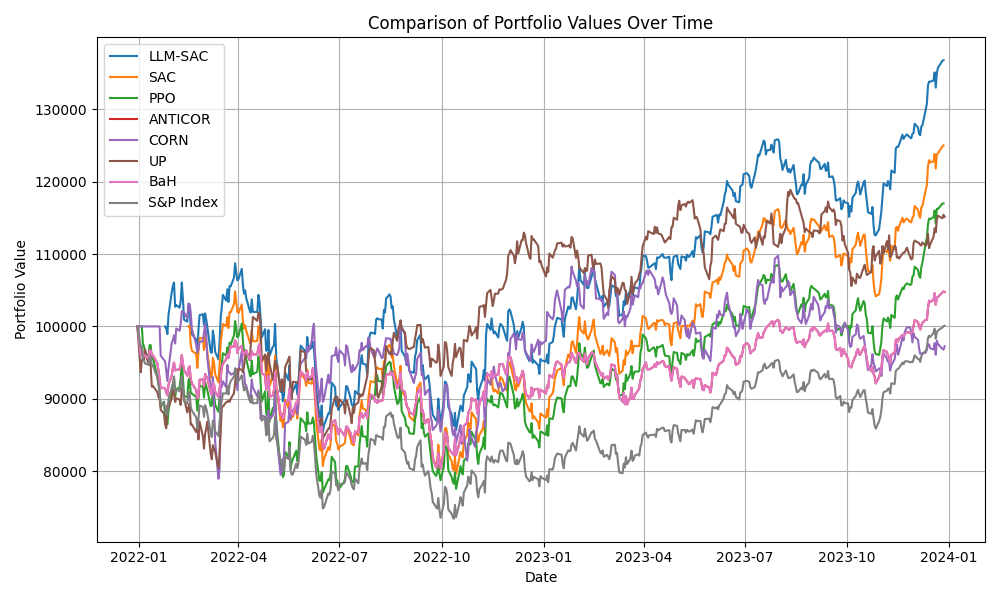
\includegraphics[width=0.8\textwidth]{images/CPV_plot.png}
  \caption{Cumulative Portfolio Value of the strategies and RL model. Our LLM-SAC model performance was able to surpass both non-LLM RL agents and strategies}
  \label{fig:portfolio_value}
\end{figure}

\csvreader[
  head to column names,
]{data/evaluation_metrics.csv}{}{
  \dimen0=\cumulative pt
  \ifdim\dimen0>\maxCumul   \global\maxCumul=\dimen0\fi
  \dimen0=\annualized pt
  \ifdim\dimen0>\maxAnn     \global\maxAnn=\dimen0\fi
  \dimen0=\sharpe pt
  \ifdim\dimen0>\maxSharpe  \global\maxSharpe=\dimen0\fi
  \dimen0=\mdd pt
  \ifdim\dimen0>\maxMDD     \global\maxMDD=\dimen0\fi
}

Turning to the \gls{RL} agents, the \gls{PPO} agent achieved a cumulative return of \(16.99\%\). The standard \gls{SAC} agent, without LLM augmentation, performed notably better, securing a cumulative return of \(24.90\%\). Both \gls{RL} agents outperformed most traditional strategies, highlighting the general advantage of adaptive learning approaches in this context. The LLM-SAC agent outperform both vanilla agent with \(11.83\%\) higher \gls{CPV} than vanilla \gls{SAC} agent.

Furthermore, Table \ref{tab:performance} measures all methods with a more comprehensive set of financial metrics. The proposed LLM-SAC agent set a new performance benchmark among all tested methods. It achieved the highest an return of \(36.73\%\) over the test period, translating to an impressive annualized return of \(11.92\%\). This superior performance is also reflected in its Sharpe Ratio of \(0.81\), which was the highest recorded, indicating better risk-adjusted returns compared to all other strategies.

\begin{table}
  \centering
  \begin{tabular}{lrrrr}
    \toprule
    Strategy & CPV (\%) & CAGR (\%)
    & SR       & MDD (\%) \\
    \midrule
    \csvreader[
      head to column names,
      late after line=\\\hline,
    ]{data/evaluation_metrics.csv}{}{
      \strategy &
      \ifdim\cumulative pt=\maxCumul   \textbf{\cumulative}   \else \cumulative   \fi &
      \ifdim\annualized pt=\maxAnn     \textbf{\annualized}   \else \annualized \fi &
      \ifdim\sharpe pt=\maxSharpe      \textbf{\sharpe}       \else \sharpe     \fi &
      \ifdim\mdd pt=\maxMDD            \textbf{\mdd}          \else \mdd        \fi
    }
  \end{tabular}
  \caption{Performance of different trading methods. The LLM-SAC agent is superior in every metrics except MDD.}
  \label{tab:performance}
\end{table}

In terms of risk, the \gls{MDD} for the LLM-SAC agent was \(-21.47\%\). While the \gls{ANTICOR} and \gls{BaH} strategies exhibited slightly lower \gls{MDD} (around \(-19.68\%\)), the LLM-SAC agent's \gls{MDD} was notably better than that of the standard SAC agent (\(-24.05\%\)) and the \gls{PPO} agent (\(-23.54\%\)). This suggests that the enhanced return of the LLM-SAC agent did not come at the expense of significantly increased downside risk compared to other RL agents. The underwater plot in Figure \ref{fig:underwater_plot} further illustrates the periods and magnitudes of these drawdowns.

\begin{figure}
  \centering
  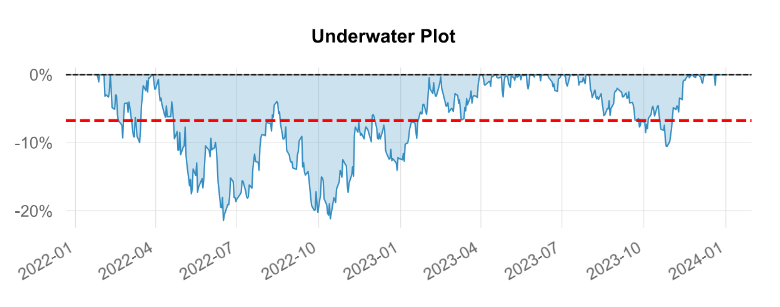
\includegraphics[width=0.8\textwidth]{images/underwater_plot.png}
  \caption{Underwater plot of LLM-SAC agent. During the beginning period, the agent suffers from significant drawdown corresponding to a bear market.}
  \label{fig:underwater_plot}
\end{figure}

Overall, these experimental findings strongly validate the hypothesis that enriching a \gls{RL} agent with \gls{LLM}‑derived sentiment signals significantly elevates trading performance. The LLM‑SAC agent not only outpaces its non‑augmented counterpart by a wide margin but also surpasses a diverse array of classic trading strategies in both absolute and risk‑adjusted terms.
